\documentclass[
  bibliography=totoc,     % Literatur im Inhaltsverzeichnis
  captions=tableheading,  % Tabellenüberschriften
  titlepage=firstiscover, % Titelseite ist Deckblatt
]{scrartcl}

% Paket float verbessern
\usepackage{scrhack}

% Warnung, falls nochmal kompiliert werden muss
\usepackage[aux]{rerunfilecheck}

% unverzichtbare Mathe-Befehle
\usepackage{amsmath}
% viele Mathe-Symbole
\usepackage{amssymb}
% Erweiterungen für amsmath
\usepackage{mathtools}

% Fonteinstellungen
\usepackage{fontspec}
% Latin Modern Fonts werden automatisch geladen
% Alternativ zum Beispiel:
%\setromanfont{Libertinus Serif}
%\setsansfont{Libertinus Sans}
%\setmonofont{Libertinus Mono}

% Wenn man andere Schriftarten gesetzt hat,
% sollte man das Seiten-Layout neu berechnen lassen
\recalctypearea{}

% deutsche Spracheinstellungen
\usepackage[ngerman]{babel}


\usepackage[
  math-style=ISO,    % ┐
  bold-style=ISO,    % │
  sans-style=italic, % │ ISO-Standard folgen
  nabla=upright,     % │
  partial=upright,   % │
  mathrm=sym,        % ┘
  warnings-off={           % ┐
    mathtools-colon,       % │ unnötige Warnungen ausschalten
    mathtools-overbracket, % │
  },                       % ┘
]{unicode-math}

% traditionelle Fonts für Mathematik
\setmathfont{Latin Modern Math}
% Alternativ zum Beispiel:
%\setmathfont{Libertinus Math}

\setmathfont{XITS Math}[range={scr, bfscr}]
\setmathfont{XITS Math}[range={cal, bfcal}, StylisticSet=1]

% Zahlen und Einheiten
\usepackage[
  locale=DE,                   % deutsche Einstellungen
  separate-uncertainty=true,   % immer Unsicherheit mit \pm
  per-mode=symbol-or-fraction, % / in inline math, fraction in display math
]{siunitx}

% chemische Formeln
\usepackage[
  version=4,
  math-greek=default, % ┐ mit unicode-math zusammenarbeiten
  text-greek=default, % ┘
]{mhchem}

% richtige Anführungszeichen
\usepackage[autostyle]{csquotes}

% schöne Brüche im Text
\usepackage{xfrac}

% Standardplatzierung für Floats einstellen
\usepackage{float}
\floatplacement{figure}{htbp}
\floatplacement{table}{htbp}

% Floats innerhalb einer Section halten
\usepackage[
  section, % Floats innerhalb der Section halten
  below,   % unterhalb der Section aber auf der selben Seite ist ok
]{placeins}

% Seite drehen für breite Tabellen: landscape Umgebung
\usepackage{pdflscape}

% Captions schöner machen.
\usepackage[
  labelfont=bf,        % Tabelle x: Abbildung y: ist jetzt fett
  font=small,          % Schrift etwas kleiner als Dokument
  width=0.9\textwidth, % maximale Breite einer Caption schmaler
]{caption}
% subfigure, subtable, subref
\usepackage{subcaption}

% Grafiken können eingebunden werden
\usepackage{graphicx}

% schöne Tabellen
\usepackage{tabularray}
\UseTblrLibrary{booktabs, siunitx}

% Verbesserungen am Schriftbild
\usepackage{microtype}

% Literaturverzeichnis
\usepackage[
  backend=biber,
]{biblatex}
% Quellendatenbank
\addbibresource{lit.bib}
\addbibresource{programme.bib}

% Hyperlinks im Dokument
\usepackage[
  german,
  unicode,        % Unicode in PDF-Attributen erlauben
  pdfusetitle,    % Titel, Autoren und Datum als PDF-Attribute
  pdfcreator={},  % ┐ PDF-Attribute säubern
  pdfproducer={}, % ┘
]{hyperref}
% erweiterte Bookmarks im PDF
\usepackage{bookmark}

% Trennung von Wörtern mit Strichen
\usepackage[shortcuts]{extdash}

\author{%
  Vincent Wirsdörfer\\%
  \href{mailto:vincent.wirsdoerfer@udo.edu}{authorA@udo.edu}%
  \and%
  Joris Daus\\%
  \href{mailto:joris.daus@udo.edu}{authorB@udo.edu}%
}
\publishers{TU Dortmund – Fakultät Physik}


\begin{document}
\section{Zielsetzung}
\label{sec:Zielsetzung}
In dem folgend protokollierten Versuch soll das Relaxationsverhalten des RC-Kreises untersucht werden. Das konkrete
Ziel besteht darin, die Zeitkonstante $\tau \vcentcolon = RC$ des Auf- bzw. Entladevorgangs des Kondensators zu bestimmen.
Ferner wird der Zusammenhang zwischen der Amplitude der Kondensatorspannug, sowie der Phasenverschiebung der Ausgangs- und
Kondensatorspannug und der Kreisfrequenz $\omega$ der Ausgangsspannung anlysiert. Zusätzlich soll gezeigt werden, unter 
welchen Voraussetzungen der RC-Kreis als Integrator arbeiten kann.

\section{Theorie}
\label{sec:Theorie}

\subsection{Relaxationsgleichung eines RC-Kreises}
Unter einem \emph{Relaxationsvorgang} wird die zeitliche Entwicklung eines Systems verstanden, welches sich aus seinem 
Ausgangszustand entfernt, nach einer gewissen Zeit jedoch nicht-oszillatorisch wieder in seinen Anfangszustand zurückkehrt.
Oftmals besteht dabei ein proportionaler Zusammenhang zwischen der Änderungsgeschwindigkeit $\frac{\symup{d}A}{\symup{d}t}$
der physikalischen Größe $A$ und der Abweichung von $A$ zum Endzustand $A\left(\infty\right)$:

\begin{equation}
\label{eqn:Proportionalitaet}
    \frac{\symup{d}A}{\symup{d}t} = c\left(A(t) - A(\infty)\right)
\end{equation}

\noindent Die Seperation der Variablen $A$ und $t$ in dieser Differentialgleichung und der Integration beider Seiten vom Zeitpunkt 0
bis zum Zeitpunkt t liefert

\begin{align}
\label{eqn:Amplitudenverlauf}
    \int_{A(0)}^{A(t)}\frac{\symup{d}\tilde{A}}{\tilde{A} - A(\infty)} &= \int_{0}^{t}c\symup{d}\tilde{t}  &\Leftrightarrow & &A(t) = A(\infty) \left(A(0) - A(\infty)\right)e^{ct}
\end{align}

\noindent Dabei muss in Gleichung \eqref{eqn:Amplitudenverlauf} $c < 0$ sein, damit die Funktion $A(t)$ beschränkt ist.
Ein beispielhafter Vorgang für ein Relaxationsverhalten wird durch die Ent- und Aufladung eines Kondensators in einem 
RC-Kreis dar.

\begin{figure}[H]
\label{fig:Ladungsvorgang}
    \centering
    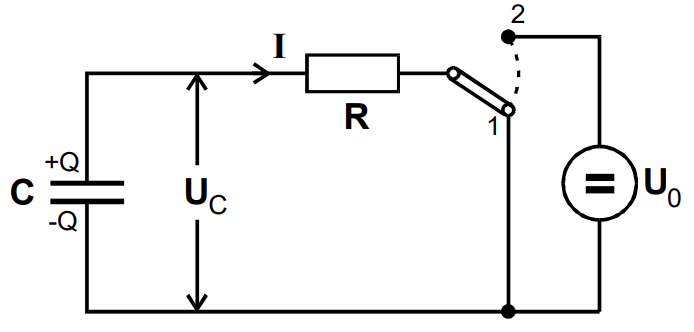
\includegraphics[height=5cm]{v353_Schaltkreise_1.png}
    \caption{Ent- und Aufladung des Kondensator.}
\end{figure}

\noindent \textbf{Entladevorgang:}\\
\noindent Wie der Abbildung \ref{fig:Ladungsvorgang} entnommen werden kann, befinden sich inverse Ladungen $Q⁺$ und $Q⁻$ auf den Platten 
des Kondensators, weswegen eine Potentialdifferenz, also eine Spannung zwischen Ihnen besteht. Diese Spannung kann mittels 
der Kapazität $C$ wie folgt ausgedrückt werden:

\begin{equation}
\label{eqn:Spannung}
    U_C = \frac{Q}{C}
\end{equation}

\noindent Um diese Potentialdifferenz wieder auszugleichen, fließen die Ladungsträger über einen ohm'schen Widerstand $R$ zur anderen Platte.
Dieser Vorgang kannn somit durch das Ohm'sche Gesetz beschrieben werden:

\begin{equation}
\label{eqn:Ohm}
    I = \frac{U_C}{R}
\end{equation}

\noindent Hierbei bezeichnet $I$ die Stromstärke. Diese ist definiert als die geflossen Ladungsmnge d$Q$ pro Zeitintervall d$t$ und kann dementsprechend
durch die Beziehung

\begin{align}
\label{eqn:Stromstaerke}
    -I &= \frac{\symup{d}Q}{\symup{d}t} &\Leftrightarrow& &\symup{d}Q = -I\symup{d}t 
\end{align}

\noindent Durch Äquivalenzumformungen und Einsetzen der Gleichungen \eqref{eqn:Spannung}, \eqref{eqn:Ohm} und \eqref{eqn:Stromstaerke} ergibt sich 
resultierend die Gleichung

\begin{equation}
    \frac{\symup{d}Q}{\symup{d}t} = -\frac{Q(t)}{RC}.
\end{equation}

\noindent Analog zur Gleichung \eqref{eqn:Proportionalitaet} wird nun eine Seperation der Variablen und die Integration beider
Seiten durchgeführt:\footnote{Hierbei wurde $Q(\infty) = 0$ angenommen, da der Kondensator nach langer Zeit
entladen ist.}

\begin{equation}
\label{eqn:}
    Q(t) = Q(0) \cdot e^{-\frac{t}{RC}}
\end{equation}

\noindent \textbf{Aufladevorgang:}\\
Gemäß der Abbildung \ref{fig:Ladungsvorgang} wird der Kondensator durch Umlegen des Schalters in Stellung 2 mittels der Spannung
$U_0$ aufgeladen. Im Gegensatz zum Entladevorgang gilt somit nun folgendes Verhalten an den Rändern:

\begin{equation*}
    Q(0) =0 \,\,\,\,\text{und}\,\,\,\, Q(\infty)= CU_0\\
\end{equation*}

\noindent Der Aufladung kann somit folgendermaßen als Funktion der Zeit formuliert werden:

\begin{equation}
    Q(t) = CU_0\left(1 - e^{-\frac{t}{RC}}\right)
\end{equation}

\subsection{Relaxationsvorgänge durch periodische Auslenkung}

Auch im Falle einer periodischen Auslenkung kann sich einer Analogie zwischen mechanischen und elektrotechnischen Systemen
bedient werden. Die mathematische Beschreibung eines durch eine periodische Kraft beeinflussten harmonischen Oszillator weist
eine Vielzahl von Parallelen zu einer sinusförmigen Wechselspannung auf. Dementsprechend wird sich im Folgende erneut auf den
RC-Kreis berufen, an welchem eine sinusförmige Wechselspannung anliegt.\\\\
Allgemein hat die Wechselspannung mit der Kreisfrequenz $\omega$ als Funktion der Zeit die Form

\begin{equation}
    U(t) = U_0\cos(\omega t).
\end{equation}

\noindent Abhängig davon, welchen Betrag die Kreisfrequenz $\omega$ der Ausgangsspannung hat, stellt sich nach gewisser Zeit eine
Phasenverschiebung $\varphi(\omega)$ zwischen der Ausgangsspannung $U(t)$ und der Kondensatorspannug $U_C(t)$ ein. Auch
die Amplitude $A(\omega)$ der Kondensatorspannug wird sich durch die Wahl von $\omega$ von der Ausgangsamplitude $U_0$ unterscheiden.
Den genauen Zusammenhang zwischen der Kreisfrequenz $\omega$ und der Phasenverschiebung $\varphi(\omega)$ sowie der Amplitude
$A(\omega)$ gilt es im Folgenden zu unteruchen.\\\\
Durch die allgemeine Abhängigkeit von der Kreisfrequenz lässt sich jedoch bereits ein Ausdruck für die Kondensatorspannug finden:

\begin{equation*}
    U_C(t) = A(\omega)\cdot\cos\left(\omega t + \varphi(\omega)\right)
\end{equation*}

\noindent Nun wird versucht konkrete Audrücke für die Terme dieser Gleichung zu finden. Mit Hilfe des zweiten Kirchhoff'schen Gesetzes

\begin{equation*}
    U(t) = U_R(t) + U_C(t),
\end{equation*}

\noindent welches besagt, dass die Summe aller Teilspannungen in einer Masche Null ergibt und der bereits aus \eqref{eqn:Spannung} und \eqref{eqn:Ohm} bekannten Äquivalenz

\begin{equation*}
    I(t) = \frac{\symup{d}Q}{\symup{d}t}= C\frac{\symup{d}U_C}{\symup{d}t}
\end{equation*}

lässt sich resultierend folgende Gleichung formulieren:

\begin{equation}
\label{eqn:Periode}
    U_0\cos(\omega t) = -A(\omega)\cdot\omega RC\sin\left(\omega t + \varphi(\omega)\right) + A(\omega)\cos\left(\omega t + \varphi(\omega)\right)
\end{equation}

\noindent Aus der Gleichung \eqref{eqn:Periode} lassen sich nun zwei Ausdrücke für kreisfrequenzabhängige Phasenverschiebung
und Amplitude der Kondensatorspannug finden:

\begin{gather}
    \varphi(\omega) = \arctan(-\omega RC)\\
    A(\omega) = \frac{U_0}{\sqrt{1 + \omega²R²C²}}
\end{gather}

\subsection{Die Funktion des RC-Kreises als Integrator}

Sind bestimmte Voraussetzungen erfüllt kann der RC-Kreis auch als Integrator dienen. Diese Voraussetzungen spiegelt sich wieder,
indem die Kreisfrequenz $\omega$ der Ausgangsspannung wesentlich kleiner als der Kehrwert der Zeitkonstante $\tau = RC$ ist $(\omega << \sfrac{1}{RC})$.
Dementsprechend kann ein proportionaler Zusammenhang zwischen $U_C(t)$ und $\int U(t)\symup{d}t$ bewiesen werden.\\
Wird erneut von der zweiten Kirchhoff'schen Regel gestartet und auf die Gleichungen \eqref{eqn:Spannung} und \eqref{eqn:Ohm} Bezug genommen, so zeigt sich

\begin{equation}
    U(t) = U_R(t) + U_C(t) = RC\frac{\symup{d}U_C}{\symup{d}t} + U_C(t).
\end{equation}

\noindent Unter Berücksichtigung der Voraussetzung $\omega << \frac{1}{RC}$ folgt letzlich

\begin{equation}
    U_C(t) = \frac{1}{RC}\int_0^t U(\tilde{t})\symup{d}\tilde{t}.
\end{equation}



\section{Fehlerrechnung}
\end{document}